\chapter{Programare Dinamic'a}
\section{Enun't}
\vspace{5mm}
\myindent
Pentru a prepara o ciorb'a bun'a pentru so'tul ei, Rodica se duce la pia't'a pentru a cump'ara ingredientele necesare. Ea are o list'a "Ingrediente.in" cu num'arul v\^anz'atorilor de legume disponibili 'si cu suma pe care o de'tine pe prima linie. Pe urm'atoarele n linii sunt ofertele fiec'arui v\^anz'ator sub forma unei perechi de tip (kg, pre't). Rodica dore'ste s'a afle folosind tehnica Program'arii Dinamice care este num'arul maxim de kilograme pe care le poate cump'ara cu to'ti banii pe care 'ii are.

\vspace{10mm}
\section{Descrierea solu'tiei probemei}
\myindent
Pentru a utiliza tehnica Program'arii dinamice, 'in aceast'a problem'a, trebuie s'a stabilim dimensiunile tabelei. Astfel liniile vor fi reprezentate de v\^anz'atori deoarece cu aceste "obiecte" vom lucra, iar coloanele vor fi reprezentate de suma cheltuit'a pentru c'a avem la dispozi'tie o sum'a maxim'a, o restric'tie. Cu acest tabel putem lua toate posibilit'a'tile 'si a'sa vom g'asi solu'tia cea mai bun'a. Astfel, 'in fiecare c\^amp al tabelei vom verifica care din cele 3 cazuri va fi cel mai bun pentru acea situa'tie. Primul caz este c\^and solu'tia precedent'a este cea mai bun'a 'si atunci vom prelua acea solu'tie. Al doilea caz este c\^and oferta v\^anz'atorului este mai rentabil'a dec\^at solu'tia precedent'a, iar al 3-lea caz este o combina'tie 'intre cele dou'a. 'In final, solu'tia se va reg'asi pe c\^ampul de pe ultima linie 'si ultima coloan'a.

\vspace{10mm}
\section{Prezentarea algoritmului de rezolvare a problemei}
\begin{lstlisting}[language=Python]
structura{
	greutate;
	pret;
} Ingredient;

int main()
	citeste n;
	citeste S;

	pentru i de la 1 la n
		citeste vanzator[i].greutate;
		citeste vanzator[i].pret;

	pentru i de la 0 la n
		pentru j de la 0 la S
			daca i = 0 sau j = 0
				continua;

			daca j < vanzator[i].pret
				dp[i][j] = dp[i - 1][j];
				continua;

			daca dp[i - 1][j] > vanzator[i].greutate
				dp[i][j] = dp[i - 1][j];

			altfel dp[i][j] = vanzator[i].greutate;

			daca(dp[i][j] < dp[i-1][j - vanzator[i].pret] 
				+ vanzator[i].greutate)

				dp[i][j] =  dp[i-1][j - vanzator[i].pret]
						+ vanzator[i].greutate;

	scrie dp[n][S];
\end{lstlisting}

\vspace{10mm}
\section{Aprecierea complexit'a'tii algoritmului propus}
\myindent
Din punct de vedere al complexit'a'tii temporale algoritmul va executa n *  S pa'si deoarece avem citirile care au O(1), avem citirea vectorului de v\^anz'atori care este intr-un for de la 1 la n, ceea ce inseamn'a O(n), avem apoi iterarea prin tabela dinamic'a care con'tine dou'a for-uri, unul de la 0 la n 'si unul de la 0 la S 'si 'in interiorul lor instructiuni care au complexitate O(1), deci avem O(S*n). Astfel vom avea O(S * n + n) = O(n * (S + 1)) = O(n * S).\\\\
\myindent
'In program exist'a variabile care au o complexitate spa'tiala de O(1), un vector care con'tine structuri cu 2 c\^ampuri care are complexitate O(2 * n) 'si o tabel'a de dimensiuni n+1 'si S+1 care va avea o complexitate spa'tiala O((n + 1) *  (S + 1)) = O(n * S). Apeluri recursive nu exist'a 'in acest program, deci complexitatea spa'tial'a r'am\^ane O(n * 2) pentru S $<$= 2 'si O(n * S) pentru S $>$ 2.\\

\vspace{10mm}
\section{Explicarea modului 'in care a fost ob'tinut'a rela'tia de recuren't'a}
\myindent
'In principiu, dac'a la linia i avem v\^anz'atorul cu oferta (kg, pret) vom avea pe aceast'a linie de la prima coloan'a p\^an'a la coloana pret solu'tia precedent'a, adic'a dp[i - 1][nr. coloan'a]. Apoi avem de verificat care din cele 3 solu'tii este cea mai bun'a. Se va compara solu'tia de la linia precedent'a cu oferta v\^anz'atorului actual 'si se va obtine o valoare maxim'a. Se verific'a apoi dac'a este mai rentabil'a cumularea greut'a'tii ofertei actuale cu solu'tia de la linia trecut'a dar sc'az\^and din coloana actual'a costul actualului v\^anz'ator.\\

\vspace{10mm}
\section{Exemplificarea aplic'arii algoritmului propus pentru un exemplu sugestiv}
\subsection{Exemplu de input}
\begin{verbatim}
Ingrediente.in
5 30
3 9
1 3
2 5
5 15
4 10

Rezultat: 11
\end{verbatim}
\newpage
\subsection{Aplicarea algoritmului}
\begin{figure}[H]
\centering
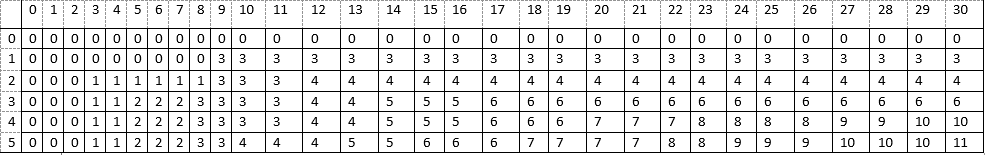
\includegraphics[scale = 0.7]{Programare Dinamica/Tabel}
\caption{Tabelul PD}
\end{figure}
\vspace{10mm}
\myindent
Dup'a citirea 'si ini'tializarea tuturor vectorilor urmeaz'a construirea solu'tiei folosind tabela PD. 'Stiind c'a tabela este ini'tializat'a la 0 nu avem nimic de modificat la linia 'si coloana cu indicele 0.\\
\newline
\myindent
Astfel, pe prima linie avem p\^an'a la costul ofertei adic'a coloana 9 solu'tia precedent'a 'si apoi vom avea doar 3 kilograme p\^an'a la final deoarece nu sunt alte oferte care s'a o precede pe aceasta. La a doua linie, la fel, p\^ana la coloana 3 solu'tia precedent'a. De la coloana 3 la 8 oferta actual'a este cea mai bun'a, deci se va trece 1 kilogram, de la 9 la 11 solu'tia precedent'a este cea mai bun'a, iar de la 12 p\^an'a la final cumularea primelor dou'a oferte va fi cea mai optim'a op'tiune.\\
\newline
\myindent
Linia a 3-a va avea p\^an'a la coloana a 4-a solu'tia precedent'a, coloanele 5 - 7 vor avea oferta actual'a, iar de la 8 'incolo se vor face cumul'ari de solu'tii. Linia a 4-a de la 0 la 19 se iau solu'tiile precedente 'si de la 20 'incolo se vor cumula ofertele, iar la linia 5 de la 0 la 9 se va lua solu'tia precedent'a, coloanele 10, 11 'si 12 vor lua oferta actual'a 'si de la 13 p\^an'a la finalul liniei se vor face cumul'ari de oferte.\\
\newline
\myindent
'In final putem extrage solu'tia de la ultima linie 'si ultima coloan'a a tabelei dp.